\documentclass{standalone}

\usepackage{tikz}
\usepackage{pgfplots}

\usetikzlibrary{arrows,shadows,positioning,shapes.geometric}
\definecolor{colone}{RGB}{62,99,118}
\definecolor{coltwo}{RGB}{82,131,156}
\definecolor{colthree}{RGB}{139,176,195}
\definecolor{colfour}{RGB}{255,211,71}

% Add layers. Add a "background" layer
\pgfdeclarelayer{bg}    % declare background layer
\pgfsetlayers{bg,main}  % set the order of the layers (main is the standard layer)

\tikzset{
  frame/.style={
    rectangle, 
    text width=8em, text centered, text = white,
    minimum height=4em,drop shadow,fill=colone,
    rounded corners,
  },
  % INPUT BOXES
  frameInput/.style={
  	trapezium,
  	trapezium left angle=60,
  	trapezium right angle=120,
  	drop shadow,
  	text width=8em,
  	text centered,
  	text = white,
  	fill = colone
  },
% Output BOXES
frameOutput/.style={
	rectangle,
	drop shadow,
	text width=10em,
	text centered,
	text = white,
	font = \sffamily\Large,
	fill = coltwo
},
  % THESIS SECTIONS
  frameSections/.style={
  rectangle,
  text width = 16em,
  text = black,
  fill = white,
  font = \sffamily\huge
  },
  % PROCESSES 
  frameProcesses/.style={
  rectangle,
  drop shadow,
  text width = 10em,
  text = white,
  fill = colthree,
  font = \sffamily\Large,
  text centered
  },
  % VARIABLE BOXES
  frameVar/.style={
  rectangle,
  text = blue!80,
  text width 8em,
  fill = white,
  text centered,
  rounded corners
  },
  % MAIN DATA FLOWS
  lineData/.style={
  draw=colfour,rounded corners=2mm,-latex
  },
  lineInfo/.style={
	draw=colfour,dashed,rounded corners=2mm,-latex
}    
}

 

\begin{document}

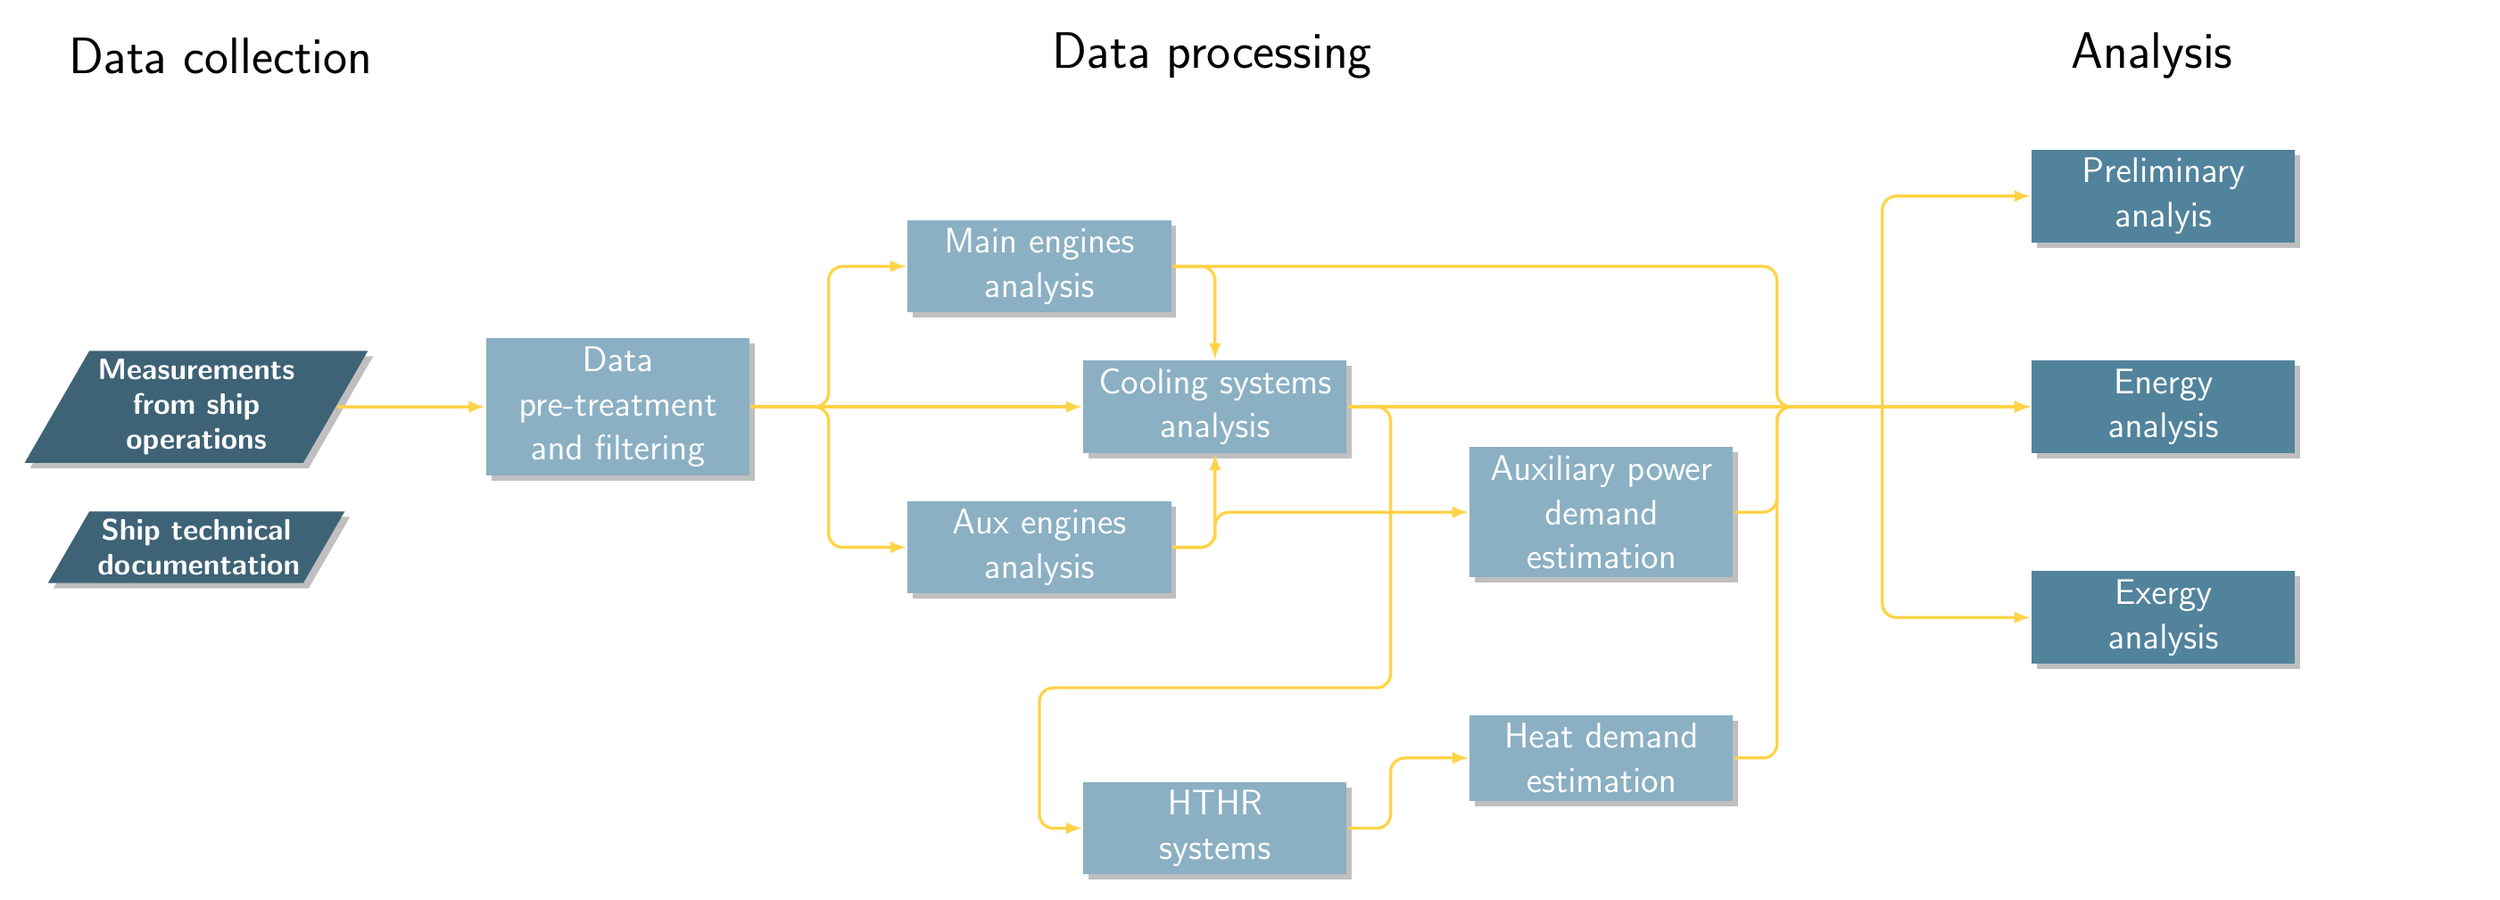
\begin{tikzpicture}[font=\large\sffamily\bfseries,very thick,node distance = 4cm]

% Input nodes for Ship 1
\node [frameInput] (input_data) at (0,-3) {Measurements \\ from ship \\ operations} ;
\node [frameInput] (input_tech) at (0,-5) {Ship technical \\ documentation} ;

% Entries on the left
\node [frameSections] (section1) at (1,2) {Data collection} ;
\node [frameSections] (section2) at (15,2) {Data processing} ;
\node [frameSections] (section3) at (29.5,2) {Analysis} ;


% Processes for ship 1
\node [frameProcesses] (process_filtering) at (6,-3) {Data \\ pre-treatment \\ and filtering} ;

\node [frameProcesses] (process_ME) at (12,-1) {Main engines \\ analysis} ;
\node [frameProcesses] (process_AE) at (12,-5) {Aux engines \\ analysis} ;
\node [frameProcesses] (process_CS) at (14.5,-3) {Cooling systems \\ analysis} ;
\node [frameProcesses] (process_HTHR) at (14.5,-9) {HTHR \\  systems} ;

\node [frameProcesses] (process_Q) at (20,-8) {Heat demand \\ estimation} ;
\node [frameProcesses] (process_Paux) at (20,-4.5) {Auxiliary power \\ demand \\ estimation} ;

\node [frameOutput] (output_preliminary) at (28,0) {Preliminary \\ analyis} ;
\node [frameOutput] (output_energy) at (28,-3) {Energy \\ analysis} ;
\node [frameOutput] (output_exergy) at (28,-6) {Exergy \\ analysis} ;


% Lines for ship 1
\path [lineData] (input_data.east) -- (process_filtering.west) ;

\path [lineData] (process_filtering.east) --  (process_CS.west) ;
\path [lineData] (process_filtering.east) -| (9,-2) |- (process_ME.west) ;
\path [lineData] (process_filtering.east) -| (9,-4) |- (process_AE.west) ;

\path [lineData] (process_CS.east) -| (17,-4) |- (15,-7) -| (12,-8.5) |- (process_HTHR.west) ;

\path [lineData] (process_AE.east) -| (14.5,-5) |- (process_Paux.west) ;
\path [lineData] (process_ME.east) -| (process_CS.north) ;
\path [lineData] (process_AE.east) -| (process_CS.south) ;
\path [lineData] (process_HTHR.east) -| (17,-8.5) |- (process_Q.west) ;

\path [lineData] (process_ME.east) -| (22.5,-2) |- (output_energy.west) ;
\path [lineData] (process_Paux.east) -| (22.5,-4) |- (output_energy.west) ;
\path [lineData] (process_Q.east) -| (22.5,-4) |- (output_energy.west) ;
\path [lineData] (process_CS.east) --  (output_energy.west) ;

\path [lineData] (24,-3) |- (output_exergy.west) ;
\path [lineData] (24,-3) |- (output_preliminary.west) ;


% LINE INFO
%\path [lineInfo] (11,-6) -| (process_AE.south) ;
%\path [lineInfo] (11,-2) -| (process_ME.south) ;
%\path [lineInfo] (13.5,-10) -| (process_HTHR.south) ;
%\path [lineInfo] (19,-9) -| (process_Q.south) ;
%\path [lineInfo] (19,-6) -| (process_Paux.south) ;
%\path [lineInfo] (input_tech.east) -| (process_filtering.south) ;

% VARIABLES
%\node [frameVar] (aa1) at (25,-2.5) {$\dot{W}, \dot{Q}$} ;
%\node [frameVar] (aa1) at (25,-5.5) {$\dot{B}$} ;
% \node [frameVar] (aa1) at (25,-6.5) {$\dot{m}, T$} ;

% Papers
%\node [framePapers] (paper1) at (8,-9) {Paper I} ;
%\node [framePapers] (paper2) at (6,-14) {Paper III} ;
%\node [framePapers] (paper3) at (13.3,-14) {Paper IV} ;
%\node [framePapers] (paper4) at (13.3,-15) {Paper V} ;




\end{tikzpicture}

\end{document}
